
% modeling Dominion in Hakaru, and what kinds of questions are interesting
% to ask the model
\section{Dominion} \label{sec:dom}

Dominion is a game we are familiar with. This game falls into the category of
{\bf turn-based
deckbuildings game}, where a player \emph{builds} a good deck by choosing what
cards to buy on their turn. The probabilistic component of deckbuilding games
arises from shuffling decks of cards at certain points in the game. In particular
in Dominion the cards a player plays can affect both when cards get shuffled
and the composition of the deck being shuffled. As a result, game-play heuristics
for Dominion are inherently intertwined with the probabilistic game state.

\subsection{Game State}

The exact details of what a model of Dominion needs to keep track of are
described in Appendix \ref{appendix:dominion-state-format}. The most important
part of this state information when formulating a buy heuristic is the set
of cards available to be bought. This set of cards is known as the \emph{supply}.
Each card in the supply has a name, a cost, and a number of copies available for
purchase. A player then, during her buy-phase, choose a card to buy costing
less than or equal to the number of \emph{treasure} cards played during her
money-phase.

In addition to the buy-phase transforming the state of the game (moving a
card from the supply into a player's discard pile), there is an action-phase
(preceding the money and buy phases) during which a player plays cards
from her hand. These cards played transform the state of the game. One
such action card which transforms the game state is described in detail
in Appendix \ref{appendix:complexcard}.

\subsection{Greedy Heuristic} \label{sec:dom:heuristics}

In Dominion a game heuristic comprises how a player plays cards, and how
she buys cards. In general the play-heuristic is easier to reason about
because it usually just involves maximization of the amount of money
in the player's hand by the end of the action phase. In probabilistic
programming terms, this can be implemented as a sampling of the
distribution over the amount of money resulting from each possible
chain of actions the player can perform. A good play heuristic might then
choose the set of actions which result in the highest expectation value
for amount of money.

For simplicity, the play-heuristic used in the experiments in this work
is one which greedily plays cards which give it more actions. After
playing all cards which give it additional actions, it plays all remaining
cards in decreasing order of cost of the card. The haskell implementation
of this is:

\begin{minted}
[ fontsize=\footnotesize
]{haskell}
greedyAct :: Game -> Measure (Maybe CardName)
greedyAct g = do 
  let as = filter isAction $ (cards.hand.p1) g
  case length as of
    0 -> return Nothing
    _ -> if elem VILLAGE as
         then return $ Just VILLAGE
         else return $ Just $ maximumBy (comparing cost) as
\end{minted}

In contrast to the play-heuristic, the buy-heuristic is a much more
interesting heuristic to study. This is because a `good' buy-heuristic
will change throughut the course of the game. Again for simplicity however,
we study a heuristic which greedily buys the most expensive card it can
with a high probability regardless of the turn number in the game. The
exact intricacies of the buy heuristic can be gleaned from the Hakaru
model implementation \cite{deckbuild-model-github}.

% -----------------------------------------------------------------------------
% Theory of the greedy-vs-greedy experiment
\subsection{Greedy Theory}
A simple query one might wish to ask of the greedy heuristic is:

\begin{quote} %\label{quote:dominion-query}
  {\bf Question 1: }
  Given that we buy card $X$ with probability $p_0$ and card $Y$ with
  probability $(1 - p_0)$, what is the distribution over the length of
  the game?
\end{quote}

In this query, we have model parameters comprising:

\begin{itemize}
\item $X$  \hsk{:: Card}
\item $Y$  \hsk{:: Card}
\item $p_0$ \hsk{:: Probability}
\end{itemize}

We also have implicit hyper-parameters comprising (see Appendix
\ref{appendix:runtime-cards} for an overview of the Haskell
implementation):

\begin{itemize}
\item \hsk{kingdomCards :: [Card]}
\item \hsk{turnRules    :: [GameParameters]}
\end{itemize}

One observe-query inference question to ask the model based on the
probable game lengths Question 1 \ignore{\ref{quote:dominion-query}} gives us is:

\begin{quote} %\label{q:inference}
%\begin{multicols}{2}
  {\bf Question 2: }
  In a greedy buy heuristic a player buys card $X$ with some unknown probability $p_0$
  and card $Y$ with probability $(1 - p_0)$. We observe a game length of $t_e'$
  turns. What is the probability $p_0$ the greedy heuristic used?
%  \columnbreak
%  (1)
%\end{multicols}
\end{quote}

The semantics of this question are slightly different than those of
Question 1 \ignore{\ref{quote:dominion-query}}. They key difference is in the
perspective of the asker. In this question $p_0$ is a latent variable
because the asker is not told the value of this parameter to the greedy
heuristic model. In the previous question $p_0$ was simply a parameter
to the model because the perspective of the question is from the player
executing the buy heuristic. See Section \ref{sec:future:PPL} for a
discussion of the linguistic ramifications of the context-dependence
of whether or not a variable is latent, observable, a parameter, or a
hyper-parameter. For the greedy model presented in this work, we do
not constrain the type of $p_0$ with any of these type abstractions.
This is primarily because Hakaru neither requires nor enforces such types.

The simplicity of this question makes for an easier to follow domain
analysis of the greedy heuristic. It however has the drawback of not being as
interesting as more complex queries. An obvious extension to this query
is to expand the state space to include a parameter $p_i$ for every possible
\hsk{(money,card) :: (Int,Card)} pair. The lack of probabilistic abstractions
just discussed however makes the implementation of such a model in Hakaru
error-prone. Therefore for the sake of ensuring correctness of our implementation,
we only present results for the one-parameter case. See the future work
section (Section \ref{sec:future:PPL}) for further discussion of the
abstractions a PPL might support.

% -----------------------------------------------------------------------------
% Results figures:
\subsection{Greedy Results \& Analysis} \label{sec:dom:greedy-results}
We now present results for the greedy heuristic, as described in
Section \ref{sec:dom:heuristics}. Before answering the inference
question (Question 2\ignore{\ref{q:inference}}), we first take unconditioned
samples from the greedy-vs-greedy model to determine characteristic
game lengths. The result of this sampling is realized as a
gaussian-like distribution of Figure \ref{fig:turn-dist}. Sampling
the model with other values of the \hsk{VILLAGE} - \hsk{CHANCELLOR}
buy ratio $p_0$ shows that $p_0$ is inversely related to the mean
of the gaussian $\mu_{t}$.

From this information we infer that the \hsk{VILLAGE} card has
a greater impact on how quickly the game ends. This is interesting
to a player of Dominion attempting to come up with a ranking of
cards. Performing an automated analysis on every possible pair
of cards using this sampling technique, one could:

\begin{itemize}
\item Design a good greedy buy heuristics
\item Determine the balance of the hyper-parameter corresponding
      to which cards are being used in the game.
\end{itemize}

The \hsk{VILLAGE} having a greater impact on the game ending is
also in line with the personal belief of the author that a
\hsk{VILLAGE} is, in general, more useful than a \hsk{CHANCELLOR}.
However, what the gaussian form of Figure \ref{fig:turn-dist}
does not tell us is the characteristic distribution of values of
$p_0$ for a given game length. This is what the inference Question
2 \ignore{\ref{q:inference}} is trying to give us insight into.

%While this is
%interesting and is in line with the personal belief of the author
%that a \hsk{VILLAGE} is generally more useful than a
%\hsk{CHANCELLOR}, it does not say anything about the characteristic
%value of $p_0$ for a given game length.

%TODO:
%figure: one column showing the un-normalized (frequency) plots of
%the rejection sampling, second column showing the normalized
%(probability density) 
%OR: one column of 3 plots, with the left-hand axis corresponding to
%frequency and the right-hand y-axis corresponding to probability.
%plot the distributions / barcharts on the same graph in different
%colors / with some alpha value.

In Figure \ref{fig:rejection-sampling} we see the characteristic
form of the turn-conditioned distribution over the
\hsk{VILLAGE} - \hsk{CHANCELLOR} buy ratio ($p_0$). At first glance
these distributions appear to be linear in $p_0$. In terms of our
parameters we can therefore write the equation:

\begin{equation} \label{eqn:linear-distribution}
P(p_0 | t_e = t_e') = m(p_0, X, Y) * p_0 + b(p_0, X, Y)
\end{equation}

In this equation we now have a name for the observed random variable
`game length' ($t_e$, the end turn number).
We also have $t_e'$ a specific (conditional) value for $t_e$.
Finally the latent random variables $m$ and $b$ together comprise a
characteristic description of the conditional distribution. The
key to this equation is that $m$ and $b$ are variables which cannot
be directly sampled / observed and have a probabilistic causal affect
on the observed variable $t_e$.
Since we have no feasible means for determining the closed analytical
forms of $m$ and $b$ we have relied on the Markov Chain Monte-Carlo (MCMC)
methods as described earlier in Section \ref{sec:mcmc}.

For the specific case of $X =$ \hsk{VILLAGE} and $Y =$ \hsk{CHANCELLOR},
we see (Figure \ref{fig:rejection-sampling}) a relationship where as the
number of turns $t_e'$ we condition on goes down...

\begin{itemize}
\item the slope $m$ of the conditional distribution increases from negative to positive
\item the intercept $b$ decreases
\item the area under the distribution gradually shifts from low values of $p_0$ to
      high values of $p_0$.
\end{itemize}

These trends are unsurprisingly in accordance with the trend of $\mu_{t_e}$,
the mean of the gaussian distribution of Figure \ref{fig:turn-dist}. Namely
that the \hsk{VILLAGE} to \hsk{CHANCELLOR} ratio increases as the number of
turns in the game decreases. The new insight we have gained from our MCMC
methods is the form of Equation \ref{eqn:linear-distribution} as well as values
for the latent variables $m$ and $b$ at various conditioned points. The form
of the conditional distribution is in fact itself a latent variable which
can be dependent on both the hyper-parameters to the game engine and parameters
to the probabilistic model. Presently it is a latent variable which can only be
computed by a human, but given a good fitting algorithm could be automated.
See Section \ref{sec:future} for further discussion of analysis automation.

% TODO: this paragraph...
variables of $t_e$ the observed game
length random variable, $t_e'$ a specific value for $t_e$, and
$m$ and $b$ the latent random variables which together comprise
a characteristic description of the conditional distribution
as described on the right-hand side of the equation.

% -----------------------------------------------------------------------------
% Results figures:

\begin{figure}
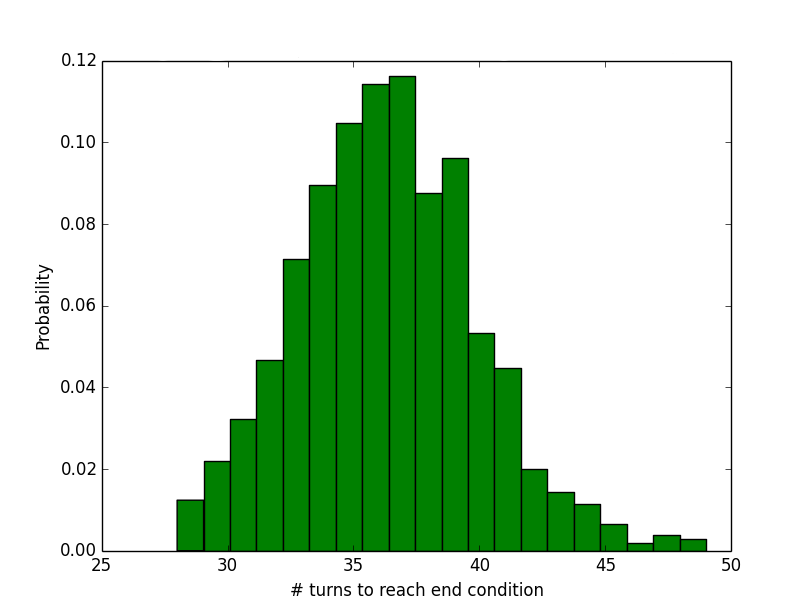
\includegraphics[width=.95\columnwidth]{../pres/village-chancellor-turn-dist.png}
\caption{\label{fig:turn-dist} Probability distribution over number of turns
in a 2-player game of Dominion.
Both players play a greedy strategy with model
parameters of $X = \textrm{Village}$, $Y = \textrm{Chancellor}$, and
$p_0 = 0.5$. See Appendix \ref{app:dominion-card} for a complete description
of the semantics behind these cards and why this pair of cards is interesting
for the game Dominion.
This distributions is unconditioned, therefore only requiring sampling directly
from the model (no inference).
}\end{figure}


% future work: less noisy / more samples / error bars on the bar charts
%               -- validate the form of the distribution statistically

\section{Probabilistic Language Analysis} \label{sec:meta-analysis}

Existing probabilistic languages seem to rely heavily on the linguistic
constructs given to them by their host languages. From our experience and
current discussion of BLOG \cite{BlOG} and Hakaru \cite{hakaru}, we see that PPLs
which tend to defer to their host language's abstraction capabilities are more
expressive and powerful. At the same time such languages also rely
heavily on the model of computation given to them by their host language.
Hakaru relies heavily on Haskell's monadic mode of computation. BLOG on
the other hand has developed the {\bf many-worlds} model of computation.

Probabilistically, the latter model of computation can be very satisfying
in terms of its similarity to the mathematical description of a probabilistic
process. In many situations declaratively
describing a probabilistic model of the possible worlds is more natural.
In the domain of games, one can envision a declarative enumeration
of the rules in a game and how they affect the game state.

Such rules form the underlying mechanics of a game. The probabilistic
components of these mechanics are, as discussed throughout this work,
implementable in PPLs. The difficulties in creating these implementations
in Hakaru in particular are described below (Section \ref{sec:hakaru-analysis}).

\subsection{Hakaru Analysis} \label{sec:hakaru-analysis}

When implementing in Haskell a complex model like that of Dominion, a
need for various monadic structures arises. In the case of Dominion
this includes the \hsk{State} and \hsk{Measure} monads (and eventually
the \hsk{IO} monad). It would therefore have been helpful for Hakaru's
\hsk{Measure} monad to support standard Haskell monads (\hsk{State} in
particular). The current implementation of our model manages to combine
these two monads using the \hsk{StateT} monad transformer and the use
of Haskell's default \hsk{lift} to move values between the \hsk{State} and
\hsk{Measure} monads. This model and more complex models using other
monads would certainly benefit from Hakaru having its \hsk{Measure}
monad derive more typeclasses.

Similarly Hakaru's interface into Haskell's random number support was
unsatisfying to use. In particular the modeler cannot specify a source
of randomness at the top-level operations Hakaru exposes. While the
default source of randomness Hakaru uses is applicable for many situations,
it makes meta-programming difficult. In the implementation of our model
we needed to re-write some of the sampling interfaces to consume a parametric
source of randomness rather than a hard-coded one in order to get the
desired effect.

Another design flaw currently baked into Hakaru's runtime system is the
use of runtime errors to unconditionally terminate the program when
Hakaru sees something it is unable to handle. The existence of
one of these errors is likely indicative of a bug in the model supplied
to Hakaru. However it is unsatisfying because it both inhibits
meta-programming and debugging.

Meta-programming is inhibited because a modeler may for instance want to
programmatically test for the correctness of a model by seeing if it
produces a runtime error. This is only feasible if the runtime error
is in some way `catchable'. Hakaru could for instance use Haskell's
\hsk{State} monad to maintain both a list of warnings and errors
along with the contents of its \hsk{Measure} monad.

Similarly runtime errors inhibit future Hakaru-specific support for
debugging because it relies on a decidedly imperative feature in a
functional host language. In particular one can modularize the implementation
of model debugging support in Hakaru if one takes advantage of the full
expressive power of Haskell in lieu of relying solely on Haskell's \hsk{error}
semantics. It would also be very helpful for Hakaru to print user-friendly
error messages and suggestions about common mistakes seen in probabilistic
models.

\subsection{BLOG Analysis} \label{sec:blog-analysis}

In addition to Hakaru we also look at the feasibility of defining a
probabilistic model of Dominion as a BLOG model. The general form
of Hakaru's issues just described in Section \ref{sec:hakaru-analysis}
is `we have a powerful host language, the abstractions
just need to be refined.' The form of BLOG's issues we discuss in this
section is `we have a powerful model of computation and a set of
natural probabilistic abstractions, but the linguistic components
of BLOG are presently undeveloped or poorly abstracted.'

One such poorly designed abstraction is the use of comprehensions
in BLOG's grammar. BLOG currently supports set-comprehensions
but not list-comprehensions. Grammatically (and syntactically) these
two features are virtually identical.
It is evident from this that BLOG's grammar has done a poor job of
distinguishing between general purpose linguistic features and
probabilistic-specific features. It is this author's opinion that
there should be a clean distinction between probabilistic and
general purpose features. BLOG in particular is, to some extent, embedded
in Java. This embedding could be exploited to a similar extent that
Hakaru exploits features of Haskell. Such an embedding would forgo the
need to `reinvent the wheel' in terms of making BLOG a more expressive
language.

The current trajectory of BLOG appears to be towards tailoring
general purpose language features to BLOG's particular model of computation.
The ambitious nature of this goal could eventually give BLOG a highly
expressive modeling form in conjunction with an efficient model of
computation. Presently however, BLOG falls significantly short of the
expressive power needed to naturally model significantly complex
probabilistic processes.


